\begin{enumerate}
    \item See Figure 1.
	\begin{figure}[h!]	
	    \centering
	    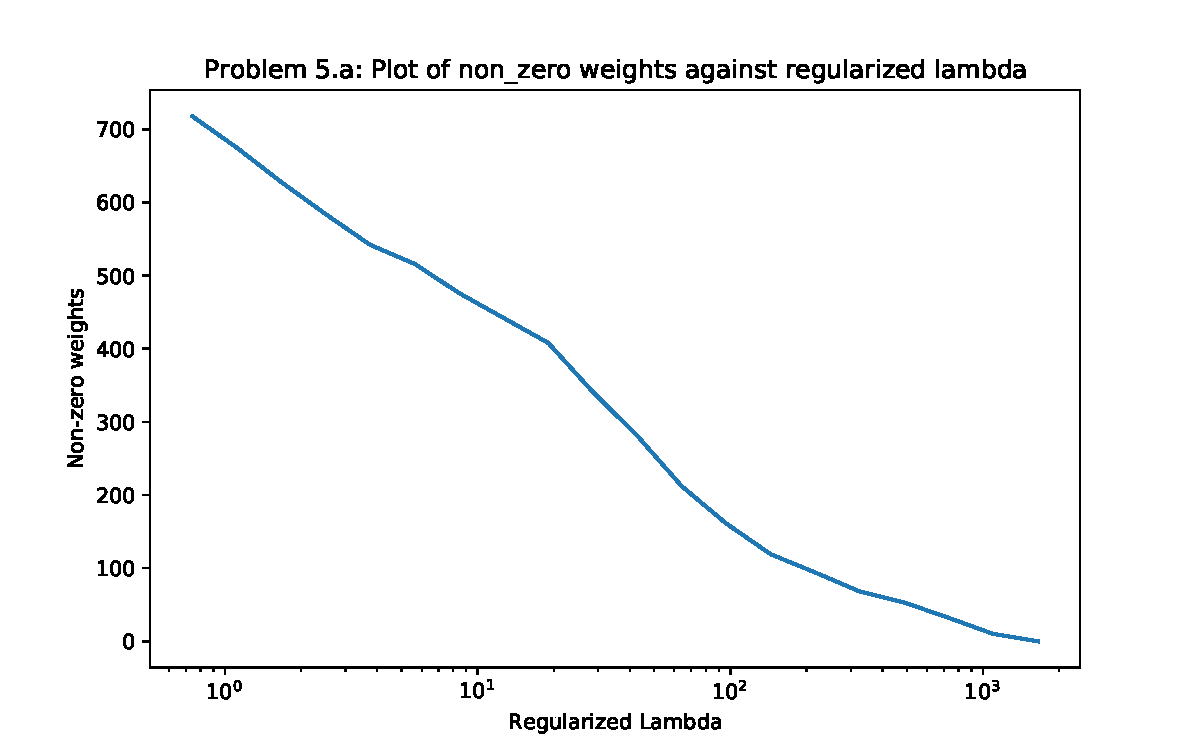
\includegraphics[width=0.5\linewidth]{images/P5_a.pdf}
	    \caption{}
	\end{figure}
    \item See Figure 2.
	\begin{figure}[h!]
	    \centering
	    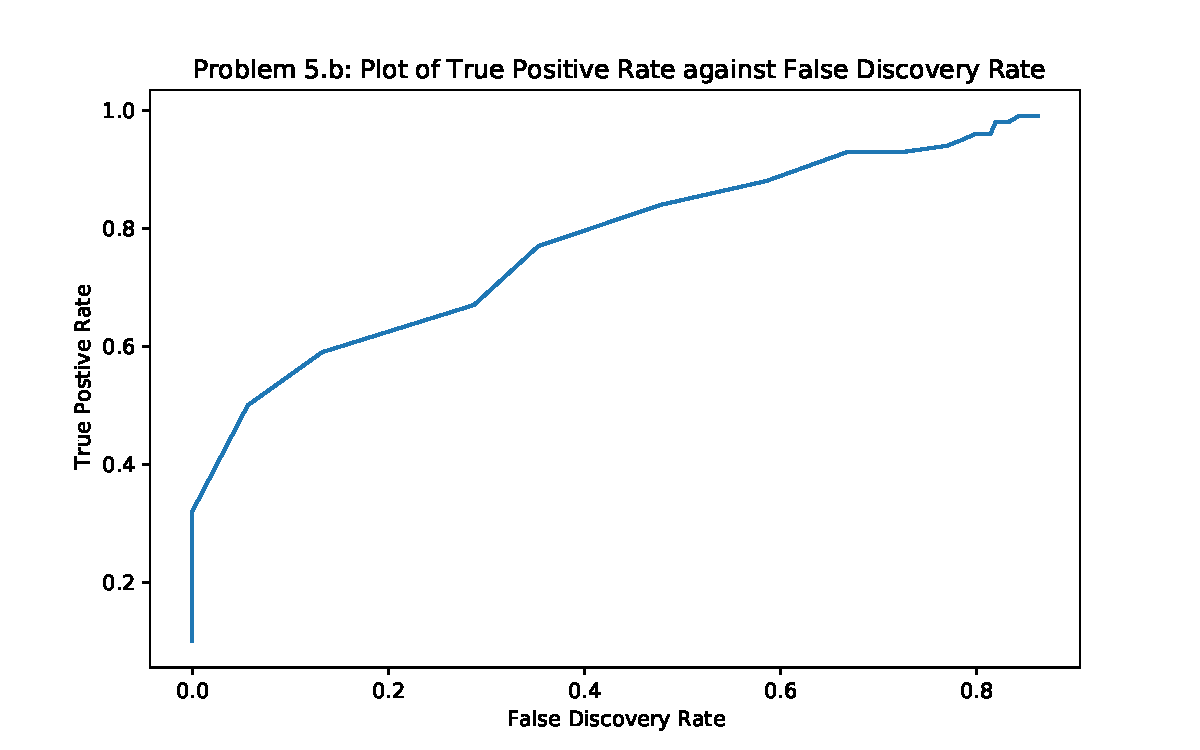
\includegraphics[width=0.5\linewidth]{images/P5_b.pdf}
	    \caption{}
	\end{figure}
    \item We see that higher $\lambda$ values increase the number of zeros in the weights leading to a more sparse solution. But we encounter problems when $\lambda$ is too small or too large. When $\lambda$ is too small, we have a hight false discovery rate and when $\lambda$ is too large the weights become too sparse and the model has poor performance. These data suggest that we should look for values of lambda that balance these trade-offs. 
\end{enumerate}
